
\section{Jenis - Jenis chipset Serial to USB}
\section{USB (Universal Serial Bus)}

\subsection{Definisi USB}
USB adalah media penghubung antara perangkat satu dengan perangkat yang lain. pada contohnya yaitu komputer dengan perangkat input outpunya yaitu Mouse, Keyboard, Flash Drive, Scanner, Dan Lain - Lain.
Teknologi USB dikembangkan pada pertengahan 1990-an ini telah menjadi standar penghubung antara komputer dengan perangkat yang mendukung. USB sendiri dapat digunakan sebagai pengisian baterai untuk perangkat - perangkat portable seperti Handphone, Power Bank, Headset Bluetooth, dan lain - lain.
USB sendiri adalah port yang sangat dipakai karena dengan bentuknya yang kecil dapat mengirim data dengan kecepatan tinggi. Yang terhubung di pada USB dapat hingga 127 perangkat dalam 1 komputer. Saat ini transfer data menggunakan USB semakin banyak, sehingga port USB menjadi pilihan utama karena kecepatan pengiriman yang besar dan ukuran yang kecil. Bus PCI sendiri sudah mendukung pengiriman data hingga 132MB/s. Konektor sendiri ada memiliki berbagai macam tetapi untuk dari perangkat ke komputer memiliki 2 macam. USB sendiri dipasang secara umum oleh banyak vendor yang membuat kemudahan dalam menghubungkan perangkat satu dengan yang lainnya. 

\subsection{Fungsi USB}
USB pada saat sekarang dapat disebut sebagai sebuah alat transceiver Baik pengirim maupun USB itu sendiri. USB sendiri terdapat yang memiliki kemampuan khusus yang dipakai ke printer, scanner, arduino, dan lain - lain. Jika data dikirim secara serial, maka USB harus mampu menangani secara kontinyu. Pada komputer sendiri, USB memiliki kemampuan dan perkembangan yang lebih baik dibanding port manapun karena efektifitasnya yang sangat tinggi.

\subsection{Perkembangan USB}
Teknologi USB sebelumnya hanya dikembangkan oleh perusahaan komputer besar seperti Intel, Microsoft, NEC yang membuat USB untuk membuat koneksi yang lebih mudah. Kabel USB sendiri menjadi standar penghubung antara komputer dengan elektronik yang membuat konektor menjadi hanya sedikit dan mempermudah dalam konfigurasi perangkat juga mempercepat transfer yang dilakukan oleh USB. USB pada komputer dapat mempercepat perangkat eksternal ke PC yang bersangkutan atau dari komputer ke perangkat elektronik tersebut.
\break
Versi pertama dari USB yaitu USB Versi 1.0 yang dirilis pada bulan Januari 1996 untuk penggunaan komersil yang memiliki kecepatan transfer data hingga 1,5 Mbit/s dan dapat mendukung 127 jenis perangkat eksternal. Untuk masa sekarang, USB sudah berkembang dan dapat 
melakukan kecepatan transfer data yang lebih tinggi yaitu berkecepatan hingga 20 Gbit/s.
\break
\begin{center}
\begin{tabular}{||c c c||} 
\hline
Versi USB & Waktu Rilis & Kecepatan Transfer \\ [0.5ex] 
\hline\hline
USB 1.0 & Januari 1996 & 1,5 Mbit/s\\ 
\hline
USB 1.1 & Agustus 1998 & 12 Mbit/s\\
\hline
USB 2.0 & April 2000 & 480 Mbit/s\\
\hline
USB 3.0 & November 2008 & 5 Gbit/s \\
\hline
USB 3.1 & Juli 2013 & 10 Gbit/s \\
\hline
USB 3.2 & September 2017 & 20 Gbit/s\\ [1ex] 
\hline
\end{tabular}
\end{center}

\subsection{Metode Transfer Data pada USB}
USB memiliki 4 metode transfer yang digunakan untuk mengirim data atau melakukan komunikasi dengan perangkat atau komputer. Metode yang terdapat pada USB diantaranya sebagai berikut : 
\begin{itemize}
\item Control Transfer \\ Metode ini digunakan untuk mengirim informasi, mengidentifikasi perangkat dan mengkonfigurasikan perangkat yang terhubung
\item Bulk Transfer \\ Metode ini mengirim data dalam jumlah besar dan memverifikasi data jika data tersebut benar atau salah. Metode ini biasa digunakan pada Printer
\item Interrupt Transfer \\ Metode ini adalah untuk mentransmisikan data kecil yang dilakukan secepat mungkin. Metode ini digunakan pada mouse atau keyboard yang selalu dipakai.
\item Isochronous Transfer \\ Metode ini digunakan untuk pemindahan data secara cepat dan realtime. Yang menjadi kunci utama pada transfer ini yaitu Waktu.
\end{itemize}
\subsection{Pengiriman data yang dilakukan USB}
Saat melakukan transfer, USB mengirim 3 paket informasi diantaranya : 
\begin{itemize}
\item Token Packet - paket yang selalu ditransfer oleh Host.
\item Data Packet - Paket yang dikirim oleh host maupun perangkat eksternal.
\item Handshake Packet - Paket yang berisi konfirmasi dari laju transfer, baik Host maupun Perangkat Eksternal dapat mengirim paket ini karena paket ini dapat mengkoreksi kesalahan yang timbul karena kesalahan transfer.
\end{itemize}
\subsection{Kelebihan Penggunaan USB}
Keuntungan yang didapat ada beberapa macam, Diantaranya : 
\begin{itemize} 
\item USB relatif mudah digunakan karena USB dapat mengkonfigurasi secara otomatis dan mendukung Single Interface untuk beberapa perangkat dan mudah dalam melakukan penambahan koneksi pada perangkat. Ukuran dari USB sendiri lebih mudah dan lebih kecil karena kabel ini hanya perlu dicolokan tanpa konfigurasi.
\item USB Memiliki kecepatan tinggi hingga 20 Mbit/s
\item USB dapat mendeteksi kesalah pengiriman data dan dapat mengirim konfirmasi dimana kesalahan dari transfer.
\item USB Memiliki biaya yang cukup murah karena penggunaannya secara luas dan massal sehingga biaya dapat ditekan sekecil mungkin.
\item Penggunaan daya lebih kecil dari kabel lainnya.
\end{itemize}
\subsection{Jenis - Jenis Connector USB}
\begin{figure}[ht]
\centerline{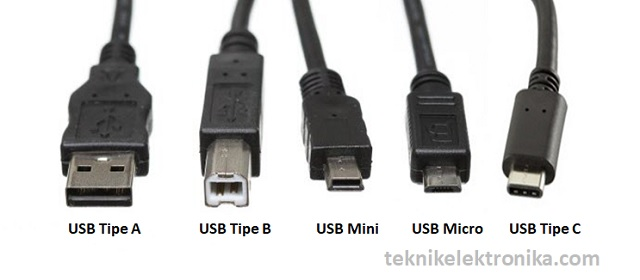
\includegraphics[width=0.6\textwidth]{figures/tipeusb.jpg}}
\caption{Tipe - tipe USB}
\label{tipeusb}
\end{figure}
Teknologi USB sudah dikembangkan mulai pada 1990-an ini telah menjadi standar penghubung antara komputer dengan perangkat yang mendukung. USB sendiri dapat digunakan sebagai pengisian baterai untuk perangkat - perangkat portable.
USB sendiri adalah port yang sangat dipakai karena dengan bentuknya yang kecil dapat mengirim data dengan kecepatan tinggi. Yang terhubung di pada USB dapat hingga 127 perangkat dalam 1 komputer. Saat ini transfer data menggunakan USB semakin banyak, sehingga port USB menjadi pilihan utama karena kecepatan pengiriman yang besar dan ukuran yang kecil. 
USB memiliki konektor yang umum digunakan, kecepatannya pun beragam setiap dari konektor tersebut. konektor itu diantaranya : 
\subsubsection{Connector Type A}
Kabel USB pada umumnya menggunakan Connector Type A (Gambar \ref{tipeusb}) baik pada perangkat komputer maupun perangkat lainnya. Connector A sendiri telah dijadikan standar dalam membuat sebuah konektor USB.
\subsubsection{Connector Type B}
Konektor ini memiliki karakteristik lekukan di kedua sudut atas. Jenis konektor ini dipakai sebagai komunikasi antara perangkat input eksternal ke komputer seperti Printer maupun Scanner.
\subsubsection{Connector Mini USB}
Konektor ini banyak digunakan pada perangkat portabel maupun ponsel sebagai media transfer maupun pengisian baterai. Konektor ini. Bentuk konektor ini lebih kecil dibanding dengan Konektor Tipe A maupun Tipe B (Gambar \ref{tipeusb}).
\subsubsection{Connector Micro USB}
Untuk Perangkat Ponsel zaman sekarang, banyak yang menggunakan Micro USB Sebagai penghubung ponsel dengan perangkat lainnya. dengan bentuknya yang tipis membuat Konektor ini digunakan oleh banyak vendor di dunia handphone.
\subsubsection{Connector Type C}
Konektor ini adalah konektor terbaru yang dapat mentransfer dengan kecepatan tinggi. Konektor ini memiliki bentuk oval dan kecil seperti Micro USB. Untuk beberapa smartphone sudah menggunakan USB Type C sebagai media transfer.
\section{Chipset}
Chipset adalah kumpulan microchip yang terdapat pada board maupun motherboard yang dibuat untuk melakukan fungsi tertentu. Fungsi dari chipset pada umumnya adalah mengatur aliran data antar komponen yang terpasang pada perangkat. Fungsi lain chipset sendiri adalah menganalisa dan mengkonfigurasi peralatan tambahan.
\subsection{Chipset North Bridge}
Chipset ini berfungsi mengatur aliran data pada peripheral internal inti.
\subsection{Chipset South Bridge}
Chipset ini mengatur aliran data pada peripheral eksternal seperti USB, Input Output, Audio, dan sebagainya.
\section{Port}
\subsection{Definisi Port}
Port adalah sebuah slot aatau colokan yang terdapat pada komputer maupun alat lain yang berfungsi untuk menghubungkan peralatan input-output atau proses. Port sendiri memiliki berbagai macam diantaranya adalah Port USB, PS/2, Serial, Parallel, dan lain - lain.
\section{Komunikasi Serial}
Komunikasi Serial atau secara ilmiah disebut RS-232 adalah standar didefinisikan sebagai interface antara perangkat terminal data dan perangkat komunikasi data atau biasa disebut DTE dan DCE. Komunikasi Serial sendiri ada pada tahun 1962 tetapi pada tahun 1997, komunikasi DTE telah diperkenalkan sebagai modifikasi standar RS-232 dan menamainya sebagai EIA-232.
Standar kecepatan dari Komunikasi Serial mencapai maksimal 256 kbps dengan jarak kurang dari 15 meter. Jenis serial sendiri dibagi menjadi dua yaitu Data Communication Equipment (DCE) dan Data Terminal Equipment(DTE). Port dari serial sendiri biasanya memiliki 9 PIN yang digunakan pada komputer ke monitor. 

Spesifikasi dari serial port mengarah pada Electronic Industry Association (EIA) : 
\begin{itemize}
\item "Space" (Logika 0) memiliki tegangan antara +3 sampai +25V.
\item "Mark" (Logika 1) memiliki tegangan antara -3 sampai -25V.
\item Daerah antara +3V sampai -3V tidak terpakai
\item Tegangan tidak boleh melebihi 25V.
\item Arus hubungan singkat tidak boleh melebihi 500mA.
\end{itemize}
\subsection{Serial RS-232}
Dulu port serial RS-232 pada komputer terdapat minimal 2 buah port. tetapi sekarang sudah berkurang menjadi 1 buah, bahkan terkadang pada komputer masa kini sudah tidak disediakan port tersebut. Hal tersebut terjadi karena teknologi yang terus berkembang, dan sudah menjadi hal yang biasa jika suatu teknologi telah ditemukan maka teknologi lama akan ditinggalkan. Walaupun begitu bukan berarti RS-232 telah ditinggalkan sepenuhnya. RS-232 sendiri memiliki kelebihan yaitu kemudahan dalam penggunaan, pemrograman yang tidak rumit, mudah untuk dipelajari dan karena sudah umum sehingga tidak sulit mendapatkan alat yang digunakan untuk merancang port serial RS-232.
\subsection{Serial DCE}
Sirkuit ini adalah perangkat yang berada di antara peralatan DTE dan rangkaian transmisi data. Hal ini biasa disebut sebagai data peralatan komunikasi atau Carrier Data Tools. Dalam proses transfer data, DCE melakukan fungsi diantaranya signal conversion, coding, dan dapat menjadi bagian dari peralatan DTE atau menengah. Perangkat ini memerlukan Interface untuk beberapa peralatan terminal data ke rangkaian transmisi atau saluran dan dari sirkuit transisi atau saluran ke DTE. Meskipun sering disebut dengan RS-232, beberapa komunikasi data berbeda definisi dengan sebutan tersebut. DCE sendiri adalah perangkat yang berkomunikasi dengan DTE dalam standar ini. Standarnya adalah sebagai berikut : 
\begin{itemize}
\item Federal Standard 1037C
\item MIL-STD-188
\item RS-232
\end{itemize}
\subsection{Serial DTE}
Sirkuit ini adalah perangkat komunikasi yang memiliki fungsi sebagai penerima sinyal dari pusat yang nanti akan dikirimkan data tersebut ke client. dimana data tersebut akan dikirimkan ke tempat yang telah ditentukan dan diterima di tempat yang ditentukan
\subsection{Fungsi dari Serial}
Komunikasi Serial atau secara ilmiah disebut RS-232 adalah standar didefinisikan sebagai interface antara perangkat terminal data dan perangkat komunikasi data atau biasa disebut DTE dan DCE. Komunikasi Serial sendiri ada pada tahun 1962 tetapi pada tahun 1997, komunikasi DTE telah diperkenalkan sebagai modifikasi standar RS-232 dan menamainya sebagai EIA-232.
Standar kecepatan dari Komunikasi Serial mencapai maksimal 256 kbps dengan jarak kurang dari 15 meter. Jenis serial sendiri dibagi menjadi dua yaitu Data Communication Equipment (DCE) dan Data Terminal Equipment(DTE).
Serial biasa digunakan untuk melakukan pengiriman data yang berpacu pada pengiriman bit per waktu, karena hal tersebut pengiriman data berjalan agak lambat. Serial sendiri biasa digunakan untuk mengkoneksikan perangkat seperti Mouse, Printer, dan lain - lain. Port yang dipakai adalah port COM. sedangkan konektor yang digunakan adalah RS-232C.
\section{Fungsi Serial to USB pada Arduino}
\subsection{Fungsi USB}
Fungsi dari konektor USB pada kabel Arduino adalah sebagai penghubung ke komputer dimana sebuah perangkat dapat dihubungkan dan dikirimkan data dari komputer ke arduino. USB sendiri dapat sebagai power supply sementara yang membuat sebuah arduino dapat dijalankan dan difungsikan juga diujicobakan. 
\subsection{Fungsi Serial}
Fungsi dari konektor Serial pada kabel Arduino adalah sebagai penerima data yang berasal dari komputer ke mikro controller Arduino yang menerima sesuai dengan kapasitas yang dapat diterima arduino. Serial sendiri memiliki kecepatan yang relatif rendah sehingga membuat pengiriman data ke arduino hanya dapat menerima dengan kecepatan cukup rendah. Pada Arduino sendiri terdapat Serial Monitor dimana data yang dikirim dari arduino dapat dilacak ke Arduino IDE pada komputer yang nanti digunakan untuk memonitor hasil yang didapat dari Arduino tersebut. Setelah dimonitor hasil yang terdapat dari arduino dapat diubah sesuai dengan tegangan serial yang dihasilkan dan disediakan oleh arduino tersebut.


